\documentclass[tikz, border=1cm]{standalone}

\usepackage{fontspec}
\setsansfont{CMU Sans Serif}%{Arial}
\setmainfont{stix}%{Times New Roman}
\setmonofont{CMU Typewriter Text}%{Consolas}
\defaultfontfeatures{Ligatures={TeX}}
\usepackage[math-style=TeX]{unicode-math}
\usepackage[english, russian, ukrainian]{babel}
\usetikzlibrary{positioning}
\usetikzlibrary{shapes.arrows}

\pgfdeclarelayer{background}
\pgfdeclarelayer{foreground}
\pgfsetlayers{background,main,foreground}

\begin{document}
\begin{tikzpicture}


\begin{scope}[shift={(-16,-8)}]
    % digit

    \newlength{\size}
    	\setlength{\size}{4cm}
    \node[inner sep=0cm, anchor=south west] at (0, 0) {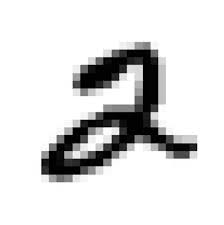
\includegraphics[width=\size]{digit.png}};

    \draw[] (0, 0) rectangle (\size, \size);

    \draw[-latex] (-0.5, \size+0.5cm) -- ++ (0, -\size-0.5cm) node[below] {$28$};
    \draw[-latex] (-0.5, \size+0.5cm) -- ++ (\size + 0.5cm, 0) node[right] {$28$};

    \foreach \i in {0,...,28} {
        \draw (0, \size*\i/28) -- ++(\size*0.03,0);
        \draw (\size, \size*\i/28) -- ++(-\size*0.03, 0);

        \draw (\size*\i/28, 0) -- ++(0, \size*0.03);
        \draw (\size*\i/28, \size) -- ++(0, -\size*0.03);
    }

    \node[draw, ultra thick, red, single arrow, text width=1cm] at (5, 2) {};
    \node[draw, ultra thick, red, single arrow, text width=1cm] at (13.5, 2) {};


    \node[font=\Large] at (9.2, 2) {
    \(    \begin{bmatrix}
    x_{11} & x_{12} & x_{13} & \cdots & x_{1, 28} \\
    x_{21} & x_{22} & x_{23} & \cdots & x_{2, 28} \\
    x_{31} & x_{32} & x_{33} & \cdots & x_{3, 28} \\
    x_{41} & x_{42} & x_{43} & \cdots & x_{4, 28} \\
    x_{51} & x_{52} & x_{53} & \cdots & x_{5, 28} \\
    \vdots & \vdots & \vdots & \ddots & \vdots \\
    x_{27, 1} & x_{27, 2} & x_{27, 3} & \cdots & x_{27, 28} \\
    x_{28, 1} & x_{28, 2} & x_{28, 3} & \cdots & x_{28, 28} \\
    \end{bmatrix}
    \)
    };

\end{scope}

	% Input Layer

	\newlength{\insize}
	\setlength{\insize}{10pt}

	\pgfmathsetmacro\nli{8}
	\pgfmathsetmacro\nlip{int(\nli - 1)}
	\definecolor{inputLayer}{rgb}{0, 0.6, 0.6}

	\begin{scope}[yshift=-1cm]
		\foreach \i in {1,...,\nlip, \nli} {

				\ifnum\i>\nlip
					\edef\s{1}
					\node[font=\large] at (0, -\i) {\ldots};
				\else
					\edef\s{0}
				\fi

				\node[circle, draw=inputLayer, ultra thick, inner sep=0pt, minimum size=\insize] (input_layer_\i) at (0, -\i-\s) {};

				\node[left=0.5cm, align=left, font=\Large] at (input_layer_\i) {
					\ifnum\i<\nli
						$x_\i$
					\else
						$x_{784}$
					\fi
				};
			}
	\end{scope}



	% First Hidden Layer

	\newlength{\firstLayerSize}
	\setlength{\firstLayerSize}{20pt}

	\pgfmathsetmacro\nlf{10}
	\pgfmathsetmacro\nlfp{\nlf - 1}
	\definecolor{firstLayer}{rgb}{0, 0, 0.6}

	\pgfmathsetmacro\xf{6}
	\begin{pgfonlayer}{foreground}
		\foreach \i in {1,...,\nlf} {


				\ifnum\i>\nlfp
					\edef\s{1}
					\node[font=\large] at (\xf, -\i) {\ldots};
				\else
					\edef\s{0}
				\fi

				\node[circle,
                draw=firstLayer,
                ultra thick,
                inner sep=2pt,
                minimum size=\firstLayerSize,
                font=\scriptsize,
                fill=white,
                text=firstLayer] (first_layer_\i) at (\xf, -\i - \s) {};

			}

	\end{pgfonlayer}
	%	\node[circle, draw=orange, inner sep=0pt, minimum size=\insize] (bias_1) at (1, -5) {};


	%	\node[below=0.5cm, align=left, orange] at (bias_1) {bias};

	% Second Hidden Layer

	\pgfmathsetmacro\nls{10}
	\pgfmathsetmacro\nlsp{\nls - 1}
	\pgfmathsetmacro\xs{9}
	\definecolor{secondLayer}{rgb}{0.6, 0, 0}



	\begin{pgfonlayer}{foreground}
		\foreach \i in {1,...,\nls} {
				\ifnum\i>\nlsp
					\edef\s{1}
					\node[font=\large] at (\xs, -\i) {\ldots};
				\else
					\edef\s{0}
				\fi

				\node[circle,
                draw=secondLayer,
                ultra thick,
                inner sep=2pt,
                minimum size=\firstLayerSize,
                font=\scriptsize,
                fill=white,
                text=secondLayer] (second_layer_\i) at (\xs, -\i - \s) {};
			}
	\end{pgfonlayer}





	% Output Layer

	\pgfmathsetmacro\xo{15}
	\definecolor{outputLayer}{rgb}{0.6, 0.6, 0.6}

	\begin{scope}[yshift=-1.5cm]
		\foreach \i in {0,...,9} {
				\node[circle,
                draw=outputLayer,
                ultra thick,
                inner sep=2pt,
                font=\large]
                (output_layer_\i) at (\xo, -\i) {$\i$};
				\node[right=0.5cm,
                font=\large] (y\i) at (output_layer_\i) {$y_\i$};
				\draw[->] (output_layer_\i) -- (y\i);
			}
	\end{scope}

	% Lines

	\foreach \i in {1,...,\nli}{
			\foreach \j in {1,...,\nlf}{
					\draw[blue!50] (input_layer_\i) -- (first_layer_\j);
				}
		}


	\foreach \i in {1,...,\nlf}{
			\foreach \j in {1,...,\nls}{
					\draw[gray!50] (first_layer_\i) -- (second_layer_\j);
				}
		}

	\foreach \i in {1,...,\nls}{
			\foreach \j in {0,...,9}{
					\draw[orange] (second_layer_\i) -- (output_layer_\j);
				}
		}

	\node[above, align=center, text width=2cm, text=firstLayer, font=\large] at (first_layer_1.north) {$128$ \\neurons};

	\node[above, align=center, text width=2cm, text=secondLayer, font=\large] at (second_layer_1.north) {$256$ \\neurons};
	%	\foreach \i in {1,...,\nlf}{
	%			\draw[orange] (bias_1) -- (first_layer_\i);
	%		}
	%
	%	\foreach \i in {1,...,\nls}{
	%			\draw[orange] (bias_2) -- (second_layer_\i);
	%		}

\end{tikzpicture}
\end{document}